\chapter{Bus Stop Detection}
\label{cha:bus-stop-detection}

The first high-level problem is the problem with inaccurate bus stop detection.
This causes the system to occasionally miss bus stops, which results in erroneous or incomplete journeys.
Incomplete journeys require more pre-processing to be done in order to use the data.
The pre-processing might also cause inaccuracies to occur in order to use the data.
An example of this is shown in Figure \ref{fig:passed-before-departed}, where a bus passes a bus stop before the system registers that the bus departed from the previous bus stop.

\begin{figure}[ht!]
    \centering
    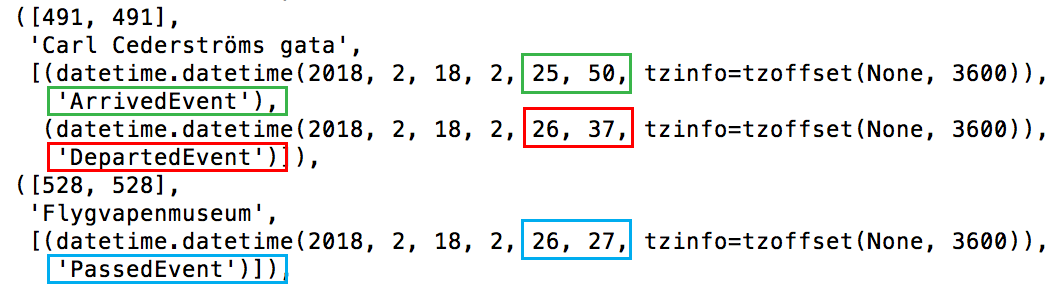
\includegraphics[width=0.9\textwidth]{figures/bad_timing}
    \caption[Example of poor bus stop detection]%
    {\small Example of poor bus stop detection. Real-world example of a bus being registered by the system to pass the "Flygvapenmusem" bus stop at 26:27,
    while it later registers the bus as having departed from "Carl Cederströms Gata" at 26:37, 10 seconds later.
    }
    \label{fig:passed-before-departed}
\end{figure}

Another problem with the existing bus stop detection algorithm is that bus stop coordinates are pre-determined, meaning that they do not always represent the actual bus stop.
This introduces an overhead to the system, where bus stop coordinates need to be updated in order to continue to provide accurate detection of bus stops.

\begin{figure}[ht!]
    \centering
    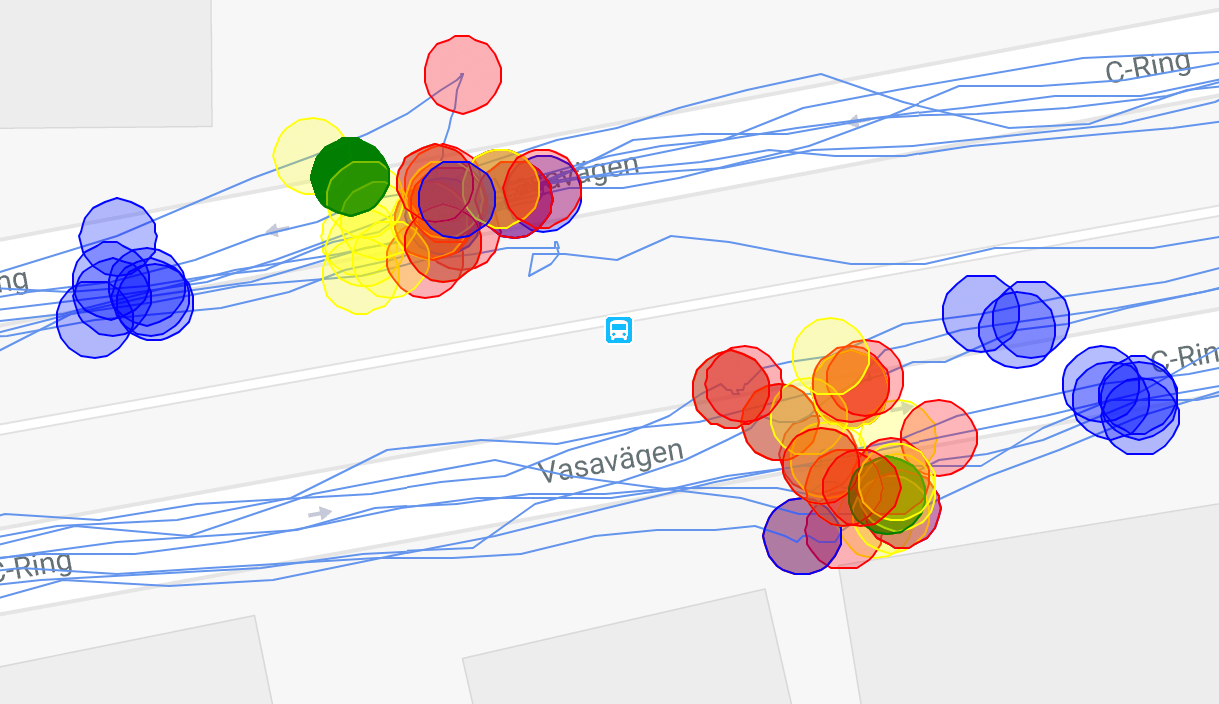
\includegraphics[width=0.9\textwidth]{figures/bus_stops}
    \caption[Output from the bus stop detection algorithm from the IA component]
    {\small Output from the bus stop detection algorithm from the IA component.
    The green circles are the pre-determined coordinates for the bus stop.
    The bus stop shown has two platforms, depending on if the bus travels west (top road) or east (bottom road).
    The red and yellow clusters are the GPS positions of the bus when it arrives to the bus stop.
    The blue clusters are the GPS positions of the buses departing from the bus stop.
    }
    \label{fig:bus-stop-clusters}
\end{figure}

Figure \ref{fig:bus-stop-clusters} shows the results from the existing bus stop detection algorithm of the IA component.
Each bus produces seven GPS coordinates for each bus stop: one blue, two red, two yellow, and one green.
\begin{itemize}
    \item \textbf{Green:} The green GPS coordinate is always the same between all buses for each bus stop; it is the pre-determined coordinate for the bus stop.
    \item \textbf{Blue:} The blue GPS coordinate is the position of the bus when it departs from the bus stop (the last positional update within a pre-determined radius of the bus stop).
    \item \textbf{Red and Yellow:} The red and yellow coordinates are the positions of the buses when the system determines that they have arrived and stopped at the bus stop.
    Due to lacking documentation, the difference between the red and yellow coordinates are unclear as they are occasionally identical, but not always (as shown in the figure).
\end{itemize}

The existing bus stop detection algorithm thus checks within a pre-determined radius around the green GPS coordinate for updates from buses.
When the first positional update from the bus is received, the system tracks the bus and waits for it to stop.
Upon stopping, the bus is determined to have arrived at the bus stop.
When the bus starts again, the system continues to track it and reports when the bus has left the radius of the bus stop.
The blue GPS coordinate shows where this happens.

\section{Methodology}
This section covers the outline on how to improve the bus stop detection algorithm.
However, due to time limitations for this thesis project, the steps in the outline will merely act as a hypothesis on how the bus stop detection can be improved.
The steps will not be implemented and the method will thus not be evaluated.

\subsection{Data Pre-Processing}
Data pre-processing is the first step required.
The procedure described in Section \ref{sec:pre-process-events} is executed in order to pre-process the data.
The result of the pre-processing step is a collection of journeys, extended with information regarding bus stops.
In addition to these results, the journeys will also be extended with \texttt{EnteredEvent} and \texttt{ExitedEvent} types.

\subsection{Dynamic Radius}
One of possible improvements to make is to introduce a dynamic radius to bus stops.
The radius could be based on analysis of the positional data from buses passing by the bus stop.
Instead of using a pre-determined radius, the radius could be decided my a model trained on observed positional data.
This only works for bus stops that detect buses approaching.

Certain bus stops are prone to be exploited by bus drivers, e.g., the example in Figure \ref{fig:stopped-before-end}.
The errors can be detected by analysing bus stops visited during a journey and compare the list against the expected list.
Manual inspection would then be required, in a pre-study step, to categorise the errors.
Some errors, like the one in Figure \ref{fig:stopped-before-end}, could be added as exceptions to the bus stop detection algorithm.
In this scenario, the bus stops and waits for a new journey assignment close to the final bus stop.
This particular scenario happens more than once throughout a single day, so it is a common bus driver behaviour.
The bus stop detection algorithm could adapt to this and increase the radius for this particular bus stop.

\subsection{Multimodal Bus Stops}
Occasionally, bus stops have space for more than one bus dropping off and picking up commuters.
This is not reflected in the dataset; the bus stops in the dataset are unimodal.
There is only one green circle for each platform of the bus stop.
An improvement to this would be to look at the stopped positions of buses at every bus stop.
The positional data would create a distribution with (longitude, latitude)-pairs denoting the different modes for each platform.
For bus stops with space for multiple buses on a single platform, the expected result would be a multimodal distribution over the actual coordinates a bus stops at.
Figure \ref{fig:multimodal-stops} shows a simulated example of a bus stop having two modes.

One of the benefits when adding information about multimodality to the system would be for the possibility of analysing the design of bus stops.
The system would produce a distribution over positions of stopped bus at each platform for each bus stop.
A multimodal distribution for a bus stop with space for only one bus would imply that the design of the bus stop could benefit by being changed.
A wide multimodal distribution could, respectively, imply the need for certain changes to the bus schedules.
For example, at specific times it could be the case that multiple buses concurrently arrive at the same bus stop, due to the nature of the time schedule.
This would cause a queue at the bus stop, or potentially unsafe loading and unloading of commuters.
A slight alteration in the schedule for a few of these buses could prevent this from occurring as often.
Arrival time prediction could be used as an assisting tool to predict bus stop queues.

\begin{figure}[t!]
    \centering
    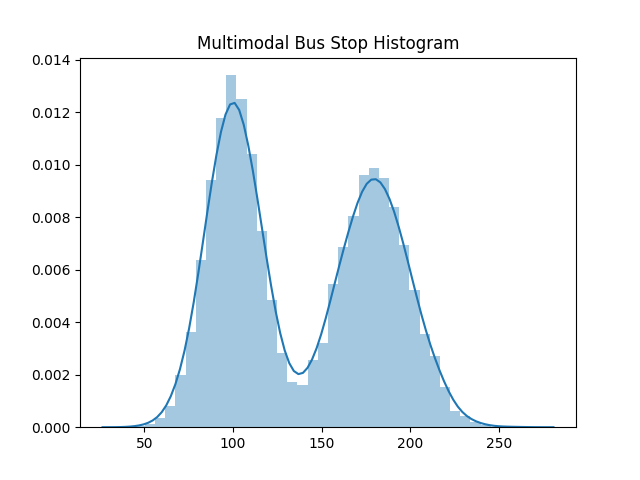
\includegraphics[width=0.9\textwidth]{figures/multimodal_bus_stops}
    \caption[Simulated example of a multimodal bus stop]%
    {{\small Simulated example of a multimodal bus stop.
    The buses mainly stop at two different positions of the platform (the two modes).
    }}
    \label{fig:multimodal-stops}
\end{figure}